\documentclass{beamer}
%\documentclass[aspectratio=169]{beamer}
\usetheme{AnnArbor}
\usecolortheme{beaver}
\usepackage[utf8]{inputenc}
\usepackage{hyperref,graphicx}
%\setbeameroption{show only notes}

\title{GIT WTF?}
\author{Björn Guth und Jörg Behrmann}
\institute[Fachschaft I/1]{Fachschaft Mathematik/Physik/Informatik der RWTH Aachen}
%\date[18.04.2013]{18. April 2013}
\titlegraphic{
\includegraphics[height=3cm]{geier.pdf}}
\logo{
\includegraphics[height=0.8cm]{geier.pdf}}


\begin{document}

\frame[plain]{\titlepage}

\begin{frame}{Inhalt}
	\tableofcontents
\end{frame}

\section{Show and Tell}
\begin{frame}{Git WTF?}
	\begin{itemize}
		\item Tool zur Versionskontrolle
		\item erleichtert kollaboratives Arbeiten
		\item einfacher Weg zu externen Backups von Projekten
		\item weiteres Argument für \LaTeX~ und gegen MS-Office / Open Office / Libreoffice
	\end{itemize}
\end{frame}

\subsection{Git im Vergleich}
\begin{frame}{Vorteile von Git gegenüber SVN}
	\begin{itemize}
		\item Git ist schneller als SVN\footnote{zumindest laut \url{http://git-scm.com/about/small-and-fast}}
		\item Git auch lokal und ohne Verbindung zu einem Server
		\item Es gibt in Git Branches
		\item SVN Repositories können in Git enigebunden werden
		\item man kann mit Git genauso arbeiten, wie mit SVN
	\end{itemize}
\end{frame}

\begin{frame}{Vorteile von Git gegenüber Dropbox}
	\begin{itemize}
		\item Git ist open source, Dropbox nicht.
		\item Dorpbox hat so gut wie keine Versionskontrolle
			\begin{itemize}
				\item Versionskontrolle nur 30 Tage
				\item alles darüber hinaus kostet Geld
			\end{itemize}
		\item Git hat .gitignore
		\item Dropbox ist ein zentralisiertes System
		\item Dropbox ist an einen Ordner gebunden
		\item viel Spaß mit den unterschiedlichen Quota der Dropboxuser
		\item Google Drive ist ähnlich einzuordnen wie Dropbox
	\end{itemize}
\end{frame}

\begin{frame}{Vorteile von Git gegenüber Dropbox}
	\begin{center}
		
\includegraphics[height=0.7\textheight]{nsa.png}
	\end{center}
	{\scriptsize Bildquelle: Wikipedia (\url{https://upload.wikimedia.org/wikipedia/commons/thumb/0/04/National_Security_Agency.svg/718px-National_Security_Agency.svg.png})}
\end{frame}

\subsection{Wie kannst man mit Git arbeiten?}
\begin{frame}{Verschiedene Möglichkeiten mit Git zu arbeiten}
	\begin{itemize}
		\item Generell gibt es drei Möglichkeiten, Git in deiner Gruppenarbeit zu nutzen:
			\begin{enumerate}
				\item Plain per ssh von Rechner zu Rechner
				\item mit Gitolite
				\item mit einen externen Hoster
			\end{enumerate}
	\end{itemize}
\end{frame}

\subsubsection{ssh}
\begin{frame}[fragile]{ssh direkt von Rechner zu Rechner}
	\begin{itemize}
		\item eine Person erstellt mit ein Repository
		\item alle anderen clonen dieses
		\item mit \verb|git remote add NAME ``ADRESSE ZUM REPOSITORY''| werden alle anderen als Quellen hinzugefügt
		\item nun können commits von anderen gepullt werden
	\end{itemize}
\end{frame}

\begin{frame}{Vor- und Nachteile}
	\begin{columns}[c]
		\column{.5\textwidth}
		Vorteile:
		\begin{itemize}
			\item dezentrales Netz
			\item alle Daten nur lokal bei euch
		\end{itemize}
		\column{.5\textwidth}
		Nachteile:
		\begin{itemize}
			\item auf jeden Rechner muss ein ssh-Daemon laufen
			\item sinnvoller Weise müsstet ihr euch dafür einen zusätzlichen User anlegen
			\item wechselnde Netzwerkadressen bereiten Probleme
		\end{itemize}
	\end{columns}
\end{frame}

\subsubsection{Gitolite}
\begin{frame}[fragile]{Gitolite zur Rechteverwaltung}
	\begin{itemize}
		\item Gitolite erledigt Rechteverwaltung bei Git-Repositories
		\item muss zusätzlich zu Git installiert und eingerichtet werden
		\item weitere Verwaltung sehr einfach über ein Git-Repository
		\item bei Interesse kann ich mehr zeigen
	\end{itemize}
\end{frame}

\begin{frame}{Vor- und Nachteile}
	\begin{columns}[c]
		\column{.5\textwidth}
		Vorteile:
		\begin{itemize}
			\item alle Daten sind lokal bei euch
			\item Rechteverwaltung sinnvoll geregelt
		\end{itemize}
		\column{.5\textwidth}
		Nachteile:
		\begin{itemize}
			\item Einrichtung nicht trivial
			\item als zentralistisches System ausgelegt\footnote{kann aber auch ähnlich wie plain ssh\\ verwendet werden}
		\end{itemize}
	\end{columns}
\end{frame}

\subsubsection{externe Hoster}
\begin{frame}{externe Hoster}
	\begin{itemize}
		\item es gibt Anbieter, die Git-Repositories zur verfügung stellen.
		\item als Beispiel seien hier mal genannt:
			\begin{itemize}
				\item github.com\footnote{bietet auch einige sehr gute Tutorials zu Git}
				\item gitorious.org
				\item bitbucket.org\footnote{bietet Git- und Murcurial-Repositories und bei Anmeldung mit einer Univeritäts-Mail-Adresse private Repositorie mit Zugriff durch soviele, wie man will.}
			\end{itemize}
		\item sehr leicht zu managen
		\item sind in der Nutzung genauso wie Gitolite
	\end{itemize}
\end{frame}

\begin{frame}{Vor- und Nachteile}
	\begin{columns}[c]
		\column{.5\textwidth}
		Vorteile:
		\begin{itemize}
			\item leichte Einrichtung
			\item vergleichsweise geringe Downtime
		\end{itemize}
		\column{.5\textwidth}
		Nachteile:
		\begin{itemize}
			\item Daten werden bösen Unternehmen in den Rachen geworfen
			\item Solange man kein Geld bezahlt, sind die Repositories public
		\end{itemize}
	\end{columns}
\end{frame}

\section{Try and (hopefully not) Fail}
\subsection{Installation}
\begin{frame}[fragile]{Installation}
	\begin{itemize}
		\item Linux:
			\begin{itemize}
				\item Mit der Paketverwaltung eurer Distribution das Paket \verb|git| installieren.
				\item Debian \& Ubuntu: \verb|sudo apt-get install git|
				\item Ansonsten: \url{http://git-scm.com/download/linux}
			\end{itemize}
		\item Windows:
			\begin{itemize}
				\item \url{https://msysgit.github.io/}
			\end{itemize}
		\item Mac OS:
			\begin{itemize}
				\item \url{http://git-scm.com/download/mac}
			\end{itemize}
	\end{itemize}
\end{frame}

\begin{frame}[fragile]{Konfiguration}
	\begin{itemize}
		\item Globale Konfiguration in \verb+~/.gitconfig+
		\item wichtige globale Konfiguratonen:
			\begin{itemize}
				\item \verb+git config --global user.name NAME+
				\item \verb+git config --global user.email EMAIL@ADREESSE+
			\end{itemize}
		\item im Projekt in \verb+./.git/config+
	\end{itemize}
\end{frame}

\subsection{usage}
\begin{frame}[fragile]{wichtigste Befehle}
	\begin{itemize}
		\item basic:
			\begin{itemize}
				\item \verb+git init+
				\item \verb+git clone ``ADRESSE ZUM REPOSITORY''+
				\item \verb+git add DATEI+
				\item \verb+git status+
				\item \verb+git commit -m ``ÄNDERUNGSBESCHREIBUNG''+
				\item \verb+git commit --amend+
				\item \verb+git push ADRESSE BRANCHNAME+
				\item \verb+git pull+
				\item \verb+git log+
			\end{itemize}
	\end{itemize}
	\begin{block}{ein eigener Versuch}
		\begin{itemize}
			\item Clont das Repository dieser Präsi
			\item \verb|git clone kiss12@137.226.113.201:~/git-vortrag|
			\item schaut mal nach, wie viele commits ich schon gemacht habe
		\end{itemize}
	\end{block}
\end{frame}

\begin{frame}[fragile]{weiter wichtige Befehle}
	\begin{itemize}
		\item more advanced:
			\begin{itemize}
				\item \verb+git branch BRANCH+
				\item \verb+git checkout BRANCH+
				\item \verb+git checkout BRANCH1+\\
					\verb+git merge BRANCH2+
				\item \verb+git diff+
				\item \verb+git branch -d BRANCH+
			\end{itemize}
	\end{itemize}
	\begin{block}{ein weiterer Versuch}
		\begin{itemize}
			\item Erstellt einen neuen Branch
			\item pusht ihn ins Repository
			\item hat es geklappt?
		\end{itemize}
	\end{block}
\end{frame}


\section{Weitere Hilfe}
\begin{frame}{Weitere Hilfe}
	\begin{itemize}
		\item \url{http://git-scm.com/doc}
		\item \url{https://help.github.com/}
		\item \url{http://wiki.ubuntuusers.de/Git}
		\item \url{http://www.markus-gattol.name/misc/mm/si/content/git_workflow_and_cheat_sheet.png}
	\end{itemize}
\end{frame}

\begin{frame}{Weitere Hilfe}
	\begin{center}
		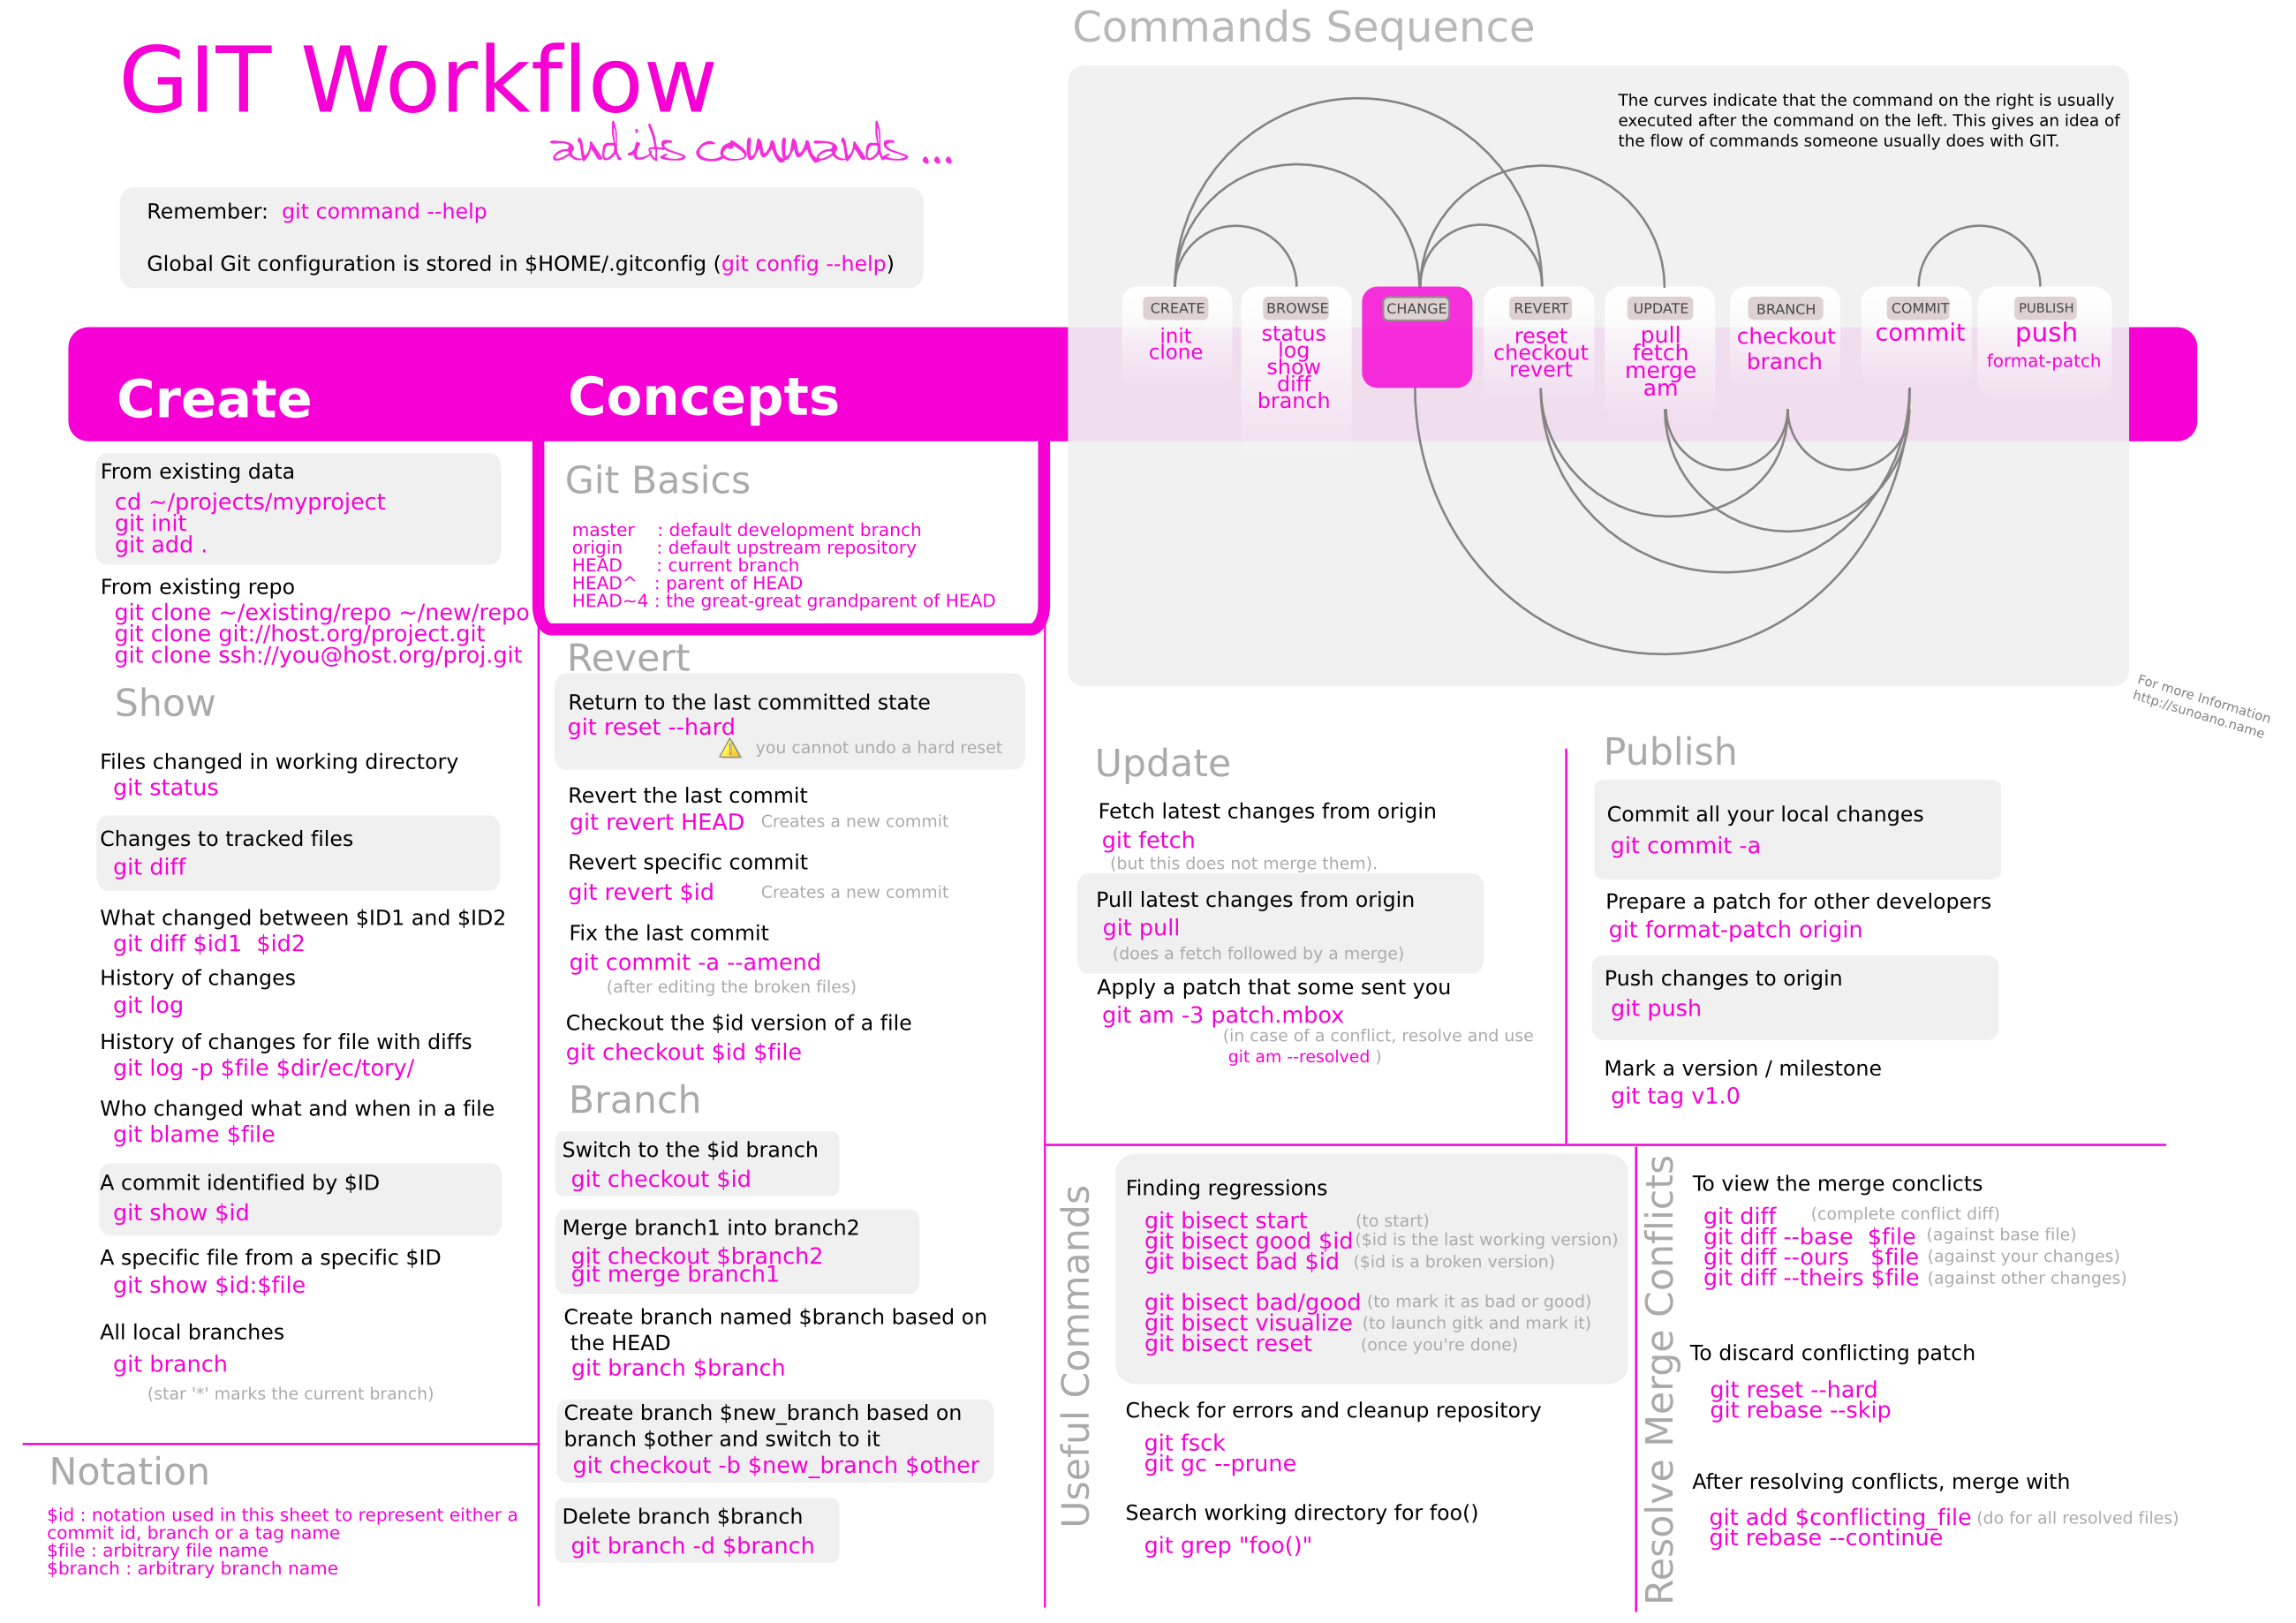
\includegraphics[height=0.7\textheight]{git_workflow_and_cheat_sheet.png}
	\end{center}
	{\footnotesize Bildquelle: Markus Gattol (\url{http://www.markus-gattol.name/misc/mm/si/content/git_workflow_and_cheat_sheet.png}}
\end{frame}

\begin{frame}
	\frametitle{Danke für die Aufmerksamkeit\footnote{auch wenn es sehr komandozeilenlastig war\footnote{}}\footnotetext{Ich hoffe aber ich konte trotzdem ein paar von euch überzeugen Git zu nutzen}}
	\begin{itemize}
		\item Wenn ihr noch Fragen habt, wäre jetzt der richtige Zeitpunkt\footnote{Später geht aber auch!}
	\end{itemize}
\end{frame}
\end{document}
